\chapter{Christologie en Chine au VIIIème siècle}

Rédaction d’une dissertation de 8 pages Vous choisissez une question
montrant comment la christologie est interrogée par une culture/autre tradition
religieuse. Vous travaillez en vous appuyant sur un article ou un autre texte.
Votre sujet et le texte doivent être au préalable validés par le professeur. Votre
travail écrit doit être déposé sur l’ENT (espace dédié) et la date limite pour la
remise de votre travail est le 8 mai 2022
Alternative regarder une approche christologique dans une culture, par exemple
perse ou chinoise. bien montrer la culture chinoise et comment elle s’adapte à
cette ”langue”, cette culture.


\section{Introduction}

Comment la christologie est interrogée par la culture chinoise au VIIIème siècle, à travers la stèle de Xi'an.

\subsection{Quel intérêt ?}
\paragraph{Une stèle du VIII} document long, écrit. 
\begin{quote}
Si les tous premiers textes que nous possédons se contentent de raconter l'histoire du Messie, il fallut bien, un jour en venir à une présentation du message chrétien dans des catégories et des perspectives proprement chinoises. C'est ce que nous fait comprendre le texte de la Stèle de Xi'an composé en 781, soit environ cent quarante ans après l'arrivée des premiers moines syro-orientaux, en 635. 
Le texte de l'inscription de la Stèle manifeste une vraie synthèse théologique qui puisait dans les trois traditions en présence, christianisme, taoïsme et bouddhisme. \cite[p.~150]{Raguin:JesusMessieXian} 
\end{quote}

\paragraph{Ecrit en très bon chinois} signe d'une compréhension fine de la culture chinoise.


\subsection{Approche}
\paragraph{Une triple difficulté pour voir l'effort d'acculturation : temps et Nestorien} En fait, la question est de savoir si cette stèle annonce la foi Chrétienne accessible à la culture chinoise ou si elle est une \textit{stèle nestorienne} présentant le christianisme sanasside. Exercice humble

\paragraph{Une approche méthodologique}



\section{Principaux traits de la culture chinoise}


\begin{Synthesis}
À retenir Primauté de l’espace dans les représentations, et des termes pratiques dans la langue. L’insertion dans les processus naturels est préférée à leur transformation selon des plans humains.
\end{Synthesis}

\cite{PolDroit:voyage} p. 115 


\paragraph{Une pensée par l'écrit} À la limite, la réflexion ne se déploie pas initialement dans l’univers de la parole, pour être ensuite transcrite, couchée par écrit, pour laisser trace. C’est plutôt dans la trace elle-même, dans la dimension de ce qui est écrit et dessiné, que s’opère le travail de la pensée. C’est en tout cas ce que suggèrent les travaux du grand sinologue Léon Vandermeersch, qui a particulièrement étudié ce phénomène des formes graphiques liées aux significations, en montrant comment la naissance des idéogrammes est liée aux observations des chamanes sur les os calcinés des sacrifices. Cette singularité expliquerait notamment pourquoi la pensée chinoise met l’accent sur les corrélations plutôt que sur les causes, et sur « le Ciel » « qui ne s’exprime pas » plutôt que sur le Verbe créateur, le logos.

 

\cite{PolDroit:voyage} p. 109 

\paragraph{La langue chinoise privilégie les termes concrets. } La plupart des mots évoquent des qualités sensibles, les vocables se rapportant à des éléments abstraits sont rares. En outre, les mots sont des « blocs », si l’on peut dire. Souvent, ils désignent une chose en même temps que telle ou telle de ses qualités (ce sont par exemple des substantifs différents qui nomment « l’eau profonde », « l’eau bouillonnante », « l’eau sale »). L’apparence n’est pas séparée de l’objet. Pareil dispositif linguistique n’incite évidemment pas à distinguer les subtances et leurs accidents…
 

\cite{PolDroit:voyage} p. 109 


\paragraph{Le ciel} Cette singularité expliquerait notamment pourquoi la pensée chinoise met l’accent sur les corrélations plutôt que sur les causes, et sur « le Ciel » « qui ne s’exprime pas » plutôt que sur le Verbe créateur, le logos.

\cite{PolDroit:voyage} p. 109 

La philosophie gréco-européenne privilégie la « forme » – en grec ancien, eïdos. Une « idée » est d’abord une « forme », qui se découpe sur un fond d’espace indifférencié. C’est ce fond d’espace qui retient l’attention chinoise, plutôt que la forme qui s’en détache. Scruter le fond plutôt que les formes, l’indifférencié plutôt que les différences, l’espace plutôt que les choses qui s’y trouvent et s’y découpent, telle pourrait être la première caractéristique de l’attitude chinoise.
Pékin. Ce lieu ne tient pas un discours sur l’espace. Il offre de l’éprouver.

\cite{PolDroit:voyage} pp. 110-111 
Il n’est pas absolument inconcevable ni tout à fait indicible. On peut en penser
et en dire quelque chose, mais cela restera toujours partiel, éphémère, incomplet. Le Ciel déborde toujours la perception qu’on en a, le récit qu’on en fait. En outre, il est changeant. Son état est mobile, et ce point est essentiel.

\cite{PolDroit:voyage} p. 111 

\paragraph{le changeant, le mobile} Il en va tout autrement du côté chinois, où le changeant, le fluent, le mobile occupent le premier plan. La tâche de la raison est de discerner ces processus de changement qui ne dépendent pas d’elle, de comprendre les transformations à venir, le plus précocément possible. L’action humaine a pour ambition de s’insérer, aussi finement qu’elle le pourra, dans les transformations de la nature.

\cite{PolDroit:voyage} pp. 112-113 

\subsection{Sagesse et religion chinoise}

\begin{Synthesis}
À retenir Entre ordre confucéen et contestation taoïste, il existe plus de complémentarité, malgré leurs désaccords, que d’opposition frontale. Ne perdant jamais de vue une dimension pratique, les débats chinois sont continûment traversés par des interrogations sur la bonté ou la méchanceté humaine, sur la bienveillance ou la cruauté nécessaire des souverains.

\cite{PolDroit:voyage} p. 147 
\end{Synthesis}

\paragraph{le sage suit le Ciel qui est en lui} Le sage suit le Ciel qui est en lui, et qui constitue le fond de notre nature. Confucius ne cesse de le répéter : à cinquante ans, il a compris comment suivre le Ciel, ce qui est identique à suivre son for intérieur. Suivre le Ciel en nous, voilà en quoi consiste la vie humaine qui se réalise pleinement.
\ldots Philo-sophia peut donc se traduire par « désir de savoir » aussi bien que par « amour de la sagesse ». C’est toujours d’un savoir acquis que dépend l’action sage. Or il n’en va pas de même quand il s’agit de suivre le Ciel. Cette fois, la vérité n’est pas un préalable.

\cite{PolDroit:voyage} p. 116 


\paragraph{éprouver le ciel} Ce n’est pas au moyen de raisonnements qu’on atteint le Ciel, qui s’éprouve directement, et il en est ainsi parce que nous sommes déjà partie prenante du Ciel et de ses transformations. Cette coexistence peut être voilée, sous-estimée, plus ou moins oubliée. Elle ne peut ni disparaître, ni être créée.

\cite{PolDroit:voyage} p. 117 


\paragraph{entrelacer moral, rites privés et gestion des affaires communes} Une caractéristique importante de la civilisation chinoise est effet d’entrelacer doctrines morales, rites privés et gestion des affaires communes.

\cite{PolDroit:voyage} p. 120 

\paragraph{Sens de l'humanité(ren)}
Car le « mandat du Ciel », comme disent les confucéens, est présent avant tout dans le « sens de l’humanité » (ren) qui habite le cœur de chacun. Cette notion fondatrice, malaisée à définir, implique à fois, selon Confucius, d’être « juste dans le jugement », « conscient de la valeur de l’effort », « pacifique dans les conflits » et d’avoir de la « retenue ». Le ren est ainsi l’instance de régulation des rapports entre les humains, agissant au cas par cas.

\cite{PolDroit:voyage} p. 122 

\paragraph{Force de la faiblesse la voie (tao)} Tao signifie, ordinairement, « la voie », « le chemin ». Très courant dans la pensée chinoise antique, le terme n’est pas propre aux « taoïstes ». Chez eux, il désigne la puissance de l’univers, la nature dans sa totalité. C’est la racine de la réalité, dans sa faiblesse et sa toute-puissance, force énigmatique d’engendrement et de destruction, en état de mutabilité permanente.\ldots explicite. Sembable au Ciel, le Tao n’est pas une chose aux arêtes distinctes. L’eau lui ressemble : « Il n’y a rien dans le monde de plus souple et plus faible que l’eau », mais elle érode les montagnes et transporte les plus lourdes charges. Elle est à la fois faiblesse extrême (goutte d’eau) et puissance sans borne (océan). \ldotsvent… C’est à force de faiblesse, si l’on ose dire, que le sage parvient à tant de puissance. L’observation de la nature l’enseigne : ce qui est faible, sans intention ni volonté propres, finit par l’emporter sur le fort, le dur, le rigide. L’eau et le vent auront raison de la montagne. Le nouveau-né commande à tous sans le vouloir ni le savoir. \ldots Ce principe ne s’atteint que par l’extase et l’intuition, ou de biais par la poésie. Car le Tao ne saurait faire l’objet d’une quête rationnelle méthodique, tout simplement parce que la rationalité, le langage et l’analyse segmentent et découpent, alors que le principe ultime est indivisible. C’est pourquoi seule l’intuition, en tant que faculté de saisie globale, embrassant la totalité d’un regard unique, peut convenir. Mais ce qu’elle fait voir et vivre n’est pas directement transmissible, seulement évocable, allusivement, par le biais d’histoires déroutantes.

\cite{PolDroit:voyage} p. 130-141 




\paragraph{Le bouddhisme} L’essor du bouddhisme en Chine, dont il sera question dans le prochain chapitre, poussera le taoïsme à se constituer en religion en adoptant son modèle, créant des ordres monastiques et des canons d’écritures sacrées. L’école Tchan naîtra en Chine d’une fusion entre taoïsme et bouddhisme, et donnera plus tard, au Japon, naissance au bouddhisme Zen (adaptation en japonais du terme chinois Tchan).

\cite{PolDroit:voyage} p. 144 


\paragraph{l'ordre} Deux termes, en chinois, disent la loi, Fa et Xing, et correspondent à deux conceptions de l’ordre. Fa, la norme, désigne la loi du Ciel, celle qui règle les phénomènes de l’univers, les cycles de la nature aussi bien que les actions humaines au sein de la société. \ldots Xing désigne la loi pénale, les châtiments prévus et administrés par le pouvoir politique pour les infractions et méfaits qui visent son autorité ou font entrave au fonctionnement de la société.



\cite{PolDroit:voyage} p. 144 

\paragraph{La Triade Taoiste Ciel-Terre-Homme}
\begin{quote}
<r Le Ciel et la Terre furent engendrés avec moi, et les Dix-mille
Êtres ne font qu ïm avec moi. Puisqu il n'y a plus que l 'Un, peut-il
y avoir discours ? Mais je viens de dire qu 'il n'y a plus que l'Un,
n'est-ce pas là du discours ? L'Un et ce que j'en dis font Deux;
le Deux afouté à l'Un fait Trois. Si l'on continue ainsi, le meilleur
des mathématiciens ne saura plus où s'arrêter; ne parlons pas du
profane. Si, en passant de l'Être à l'existant, on arrive déjà à Trois,
qu 'en sera-t-il si on passe de l'existant à l'existant ? Mieux vaut ne
passer de rien à rien, et laisser les choses comme elles sont ! »
(Zhuangzi, ch.2)
Le Trois comme facteur d'harmonie entre l'Un et le Multiple. L'idée du Trois en Chine est à replacer au sein d'une conception
du monde cosmique et moral sans Dieu créateur au centre de sa
création, ni Au-delà posé a priori. On peut ajouter que dans une
telle conception, c'est précisément le Trois qui permet de « courtcircuiter
» la référence à Dieu ou à quelque instance supra-cosmique. \sn{Cheng Anne. De la place de l'homme dans l'univers : la conception de la triade Ciel-Terre-Homme à la fin de l'antiquité
chinoise. In: Extrême-Orient, Extrême-Occident, 1983, n°3. le rapport à la nature : notes diverses. pp. 11-22.
doi : 10.3406/oroc.1983.893
http://www.persee.fr/doc/oroc_0754-5010_1983_num_3_3_893
}
\end{quote}

\subsection{ce qui parait être des caractéristiques sannaside}

\section{Analyse du texte}

\paragraph{25 sections} Le texte peut être séparé en 25 sections \cite{Pauthier:linscriptionSinganfou,p.24}
\begin{itemize}
    \item  I et 2. - Des.attributs de Dieu un et troia, dont le nom est Éloha. La création du monde tirée du néant. Le signe de la croix pris comme emblème de pacification universelle.
    \item 3. Création de l'homme; sa nature.
    \item 4. Sa chute. 
    \item 5. Naissance des sectes nombreuses qui ont agité le monde. 
    \item 6. L'incarnation; le Messie; la Vierge enfante le Saint en Syrie; une étoile annonce l'heureux évènement
; les Mages de la Perse. 
    \item 7. Accomplissement des prophéties; dogme de la Trinité; la mort vaincue par la résurrection du Saint; son ascension; les
livres qui renferment da doctrine. 
    \item 8. Institution du baptême. Le sceau du nouveau
pacte est le signe de la croix t; l'appel des fidèles frappé sur des tablettes
de bois, à la manière orientale, où les cloches ne sont pas en usage. 
    \item 9. Caractère
distinctif des apôtres de la foi nouvelle ; leur barbe, leur tonsure; ce qu'elles
signifient; ils n'ont point d'esclaves à leur service; tous les hommes sont égaux
pour eux; leur mépris des richesses. Le jeûne. La retraite. Ils prient sept fois le
jour, et offrent le premier des sept jours un sacrifice sans victimes.
    \item 10. Caractère
de la loi nouvelle, nommée la \textit{Religion resplendissante comme la lumière du
soleil }:King kiao. La loi sans les souverains; les souverains sans la loi. 
    \item
11. Arrivée d'Olopen.en Chine, venant de la Syrie, et portant avec lui les saintes
Écritures. Honneurs qui lui sont rendus. Les saintes Écritures sont portées au
palais de !'Empereur, où elles sont étudiées et trouvées excellentes. li est ordonné
de les traduire et de les enseigner en public. 
\item 12. Édit de l'Empereur Thaïtsoûng
(638) concernant la religion chrétienne. 
\item 13. Les magistrats reçoivent
l'ordre de faire faire le portrait de l'Empereur pour le placer dans l'église chrétienne.
\item14. Description de la Syrie, selon les relations chinoises
\item 15. Progrès
de la religion chrétienne en Chine sous l'Empereur Kdo-tsouug (650-683).
\item 16. Les bouddhistes et les lettrés cherchent à entraver ces progrès ; des personnages éminents, dont les uns sont venus de la tartarie, soutiennent la foi
nouvelle. 
\item 17. L'Empereur Hioûen-tsoung (713\item7 55) ordonne à cinq princes,
ses frères, d'aller visiter l'église chrétienne qu'il fait restaurer à ses frais.
\item 18. Le
même souverain fait transporter les portraits des cinq Empereurs, ses prédécesseurs,
dans l'église chrétienne; il fait don en même temps de cent pièces d'étoffe
de soie. 
\item 19. Arrivée en Chine d'un nouveau prêtre syrien. Il est invité, ainsi
que six autres prêtres chrétiens, à se rendre au palais de !'Empereur pour y accomplir les cérémonies de leur culte. L'Empereur leur donne des inscriptions morales
écrites de sa mano, et qui sont placées dans l'enceinte de l'église chrétienne.

\item 20. L'Empereur Sou-tsoung,dng (756-762) fait construire de nouvelles églises chrétiennes. 
\item 2 t. L'Empereur Tai-tsoung (763-779) envoie aux prêtres chrétiens,
à chaque jour anniversaire de sa naissance, de l'encens et des mets de sa table.
\item 22. L'Empereur Te-tsoung (780-783); éloge enthousiaste de cet Empereur.
\item 23. La vie est un écho qui répond à un autre écho. 
\item 24. Bonze indien élevé
à de hauts emplois; son éloge; ses grands talents; sa charité. Vers laudatifs,
en seize strophes, résumant le préambule qui précède. 
\item 25. Date de l'inscription,
septième jour du mois du printemps, de l'année 781 de notre ère, jour férié
de la célébration de l'Hosanna.
\end{itemize}

\paragraph{Titre}
traduction  \cite{Havret:stelechretienne}
\begin{figure}
    \centering
    \sidecaption{Titre de l'inscription \cite{Pauthier:linscriptionSinganfou} Monument (rappelant) la propagation à travers l'Empire du Milieur de l'Illustre (King) Religion du Ta-ts'in}
    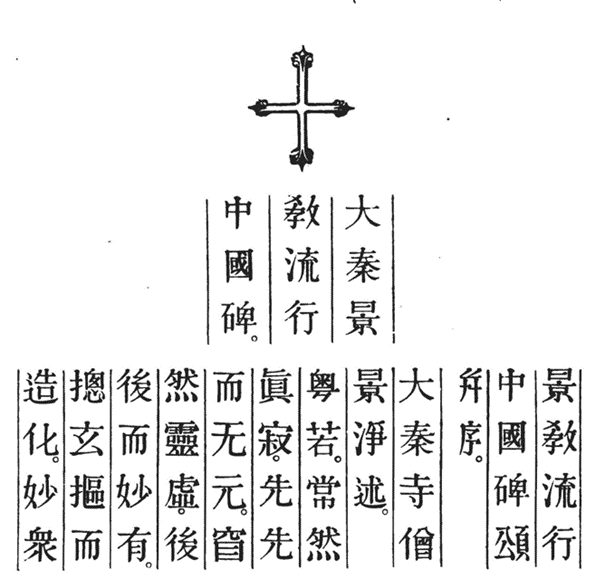
\includegraphics[width=\textwidth]{ChristologieCultureHistoire/Images/PremierParagrapheStele.png}
 
    \label{fig:my_label}
\end{figure}

\paragraph{Dieu exprimé avec les catégories Taoistes} 
\begin{quote}
    En vérité, immuable en son mode et souverainement paisible,
devançant toute origine,
lui-même sans principe ; inaccessible et
pur esprit, survivant à toute fin, dans son
admirable essence. Détenant en ses mains
une mystérieuse puissance, et auteur de la
création; admirable dans ses saints, lui le
premier digne d'hommages ; il n'est autre
que l'admirable substance de notre Trinité
une, que le vrai Seigneur sans principe.

\end{quote} 

\begin{table}[h!]
\begin{tabular}{p{5cm}p{5cm}}
Eternellement et profondément Vérité et Repos, Il précède tout ce qui est ancien. & En vérité, immuable en son mode et souverainement paisible,  devançant toute origine, lui-même sans principe ; inaccessible et  pur esprit, survivant à toute fin, dans son  admirable essence. Détenant en ses mains  une mystérieuse puissance, et auteur de la création; admirable dans ses saints, lui le  premier digne d'hommages ; il n'est autre  que l'admirable substance de notre Trinité  une, que le vrai Seigneur sans principe.  \\
                                                  &               \\
\end{tabular}
\end{table}
La forme (4 phrases parallèles deux à deux) est inspirée de divers passages du Tao-té-King de Lao-tse : le Tao est cause première,  et lui sont prêtés les attributs d'éternité, de vérité, de tranquillité, d'antériorité, d'intelligence, de profondeur, de spiritualité, de mystérieuse causalité de tous les êtres, et de Dignité. \sn{\cite{Havret:stelechretienne}, p. 11}
Au point que King-tsing, l'écrivain de la stèle a pu être qualifié comme :
\begin{quote}
    C'est un homme habile mais porté par la secte de \textit{Tao} \sn{P. Gaubil, Mémoires concernant les Chinois, Tom. XVI, 1811, p. 371.}
\end{quote}

\paragraph{Trinité}
\begin{quote} Le terme employé pour désigner la Trinité est un terme taoïste, \emph{sanyi} le "Trois-Un". mais pour signifier qu'il s'agissait de la Trinité Chrétienne, l'auteur de l'inscription a ajuté le caractère "\emph{Wo}" qui signifie "notre". Ainsi le terme taoïste a pris un sens chrétien, "Notre Trois-Un".
    \cite[p.43]{Raguin:JesusMessieXian}
\end{quote}

\begin{quote}
    Pour expliquer l'incarnation de l'un de
de ces "Trois-un", le terme employé est emprunté au bouddhisme, \emph{fenshen}. Quand un être spirituel, comme un Bouddha, veut se manifester dans le monde il se "divise" pour apparaître sous une forme visible. Cette notion n'est pas sans analogie avec la conception de la métamorphose dans la religion grecque ancienne. Le Messie apparaît donc sur terre en cachant sa divinité. ici les perspectives sont différentes de celles de Saint Paul pour qui le verbe "s'est vidé" de ses prérogatives.  \cite[p.43]{Raguin:JesusMessieXian}
\end{quote}
\begin{quote}
    Pour exprimer la relation entre le Messie personne divine incarnée, et Dieu, le terme le plus souvent employé est un terme du langage commun, mais plein de sens, "\emph{tong}" qui veut dire : communiquer, être en parfaite communion avec. [\ldots] Une hymne est tout entière consacrée au "retour à sa vraie nature" de Celui qui est en parfaite communion avec le Grand Saint (J. titre). [\ldots] le Messie est vraiment Dieu. Il est toujours là où est Dieu (C. 74). Dans un texte, le Messie est appelé "zun'er", le fils du vénéré (E. 72) \cite[p.43]{Raguin:JesusMessieXian}
\end{quote}


\section{Christologie implicite}

\paragraph{Une approche religieuse et non philosophique} qui ne sera pas retenu par M. Ricci. Influence du bouddhisme et du Taoisme. Cela peut être lié au fait que la Taoïsme était plutot une philosophie avant d'entrer en contact avec le Bouddhisme ? A creuser.


% ------------------------
\section{Chrétiens sanassides}

\subsection{Christelle Jullien. « Les chrétiens en Iran
sassanide »
}
\href{https://go.exlibris.link/YnGJKmGb}{Les chrétiens en Iran sassanide}
Le Coran des historiens
Amir-Moezzi, Mohammad Ali (1956-....)

2019

 "Première mondiale, ce monument savant et accessible, qui réunit trente spécialistes internationaux, offre, en trois mille pages, une synthèse complète et critique des travaux passés et des recherches présentes sur les origines du Coran, sa formation et son apparition, sa composition et sa canonisation : vingt études exhaustives sur le contexte introduisent ici à l'analyse circonstanciée du texte, les éléments archéologiques et épigraphiques, les environnements géographiques et linguistiques, les faits ethnologiques et politiques, les parallèles religieux éclairant, verset après verset, en un commentaire total les cent quatorze sourates du livre fondateur de l'islam. Une aventure inédite de l'esprit. Une somme sans précédent dans l'histoire. Une contribution majeure à la science. Une avancée décisive pour la compréhension mutuelle des cultures." : éditeur

\paragraph{critique} Le chapitre dévolu aux chrétiens en Iran sassanide s’intègre dans le tome 1, et participe à l’objectif de ce volume : dresser un tableau d’ensemble cherchant à mieux faire comprendre le milieu de genèse du corpus coranique. L’A. souligne que les communautés chrétiennes syriaques de l’empire iranien n’ont jamais constitué une culture dominante : mises au défi de l’intégration dans des milieux culturels et socio-politiques non chrétiens, le monde mazdéen, que relaya le monde musulman. À l’arrivée de l’islam, elles sont marquées par la pluralité du fait de leurs choix doctrinaux, faisant suite aux grandes définitions conciliaires autour de la personne et de la nature du Christ. Une première partie porte sur les premiers indices d’une présence chrétienne et sur les traditions d’évangélisation. La littérature syriaque se fait l’écho des liens étroits entre milieu missionnaire et monde marchand laïc, support des initiatives de pénétration doctrinale. La seconde a trait aux déportations en Perse et leur incidence sur le développement des communautés sur le territoire. L’appropriation des savoir-faire était l’un des objectifs premiers de ces transferts de populations au cœur de l’empire. L’A. rappelle bien la mixité culturelle des communautés chrétiennes de Perse, reflet des sociétés en monde iranien. Les autres parties abordent la question des persécutions sous l’influence progressive du clergé mazdéen au sein des organes de pouvoir, et de la nécessaire loyauté politique des chrétiens en milieu mazdéen alors que les choix christologiques des Églises exacerbent les tensions de part et d’autre de la frontière. Après un éclairage bien synthétique sur l’organisation des communautés dyophysites et miaphysites en territoire iranien et la progressive évolution de l’Église syro-orientale vers l’autonomie, le thème des controverses inter-religieuses vient à propos éclairer les succès de l’implantation de l’islam, qu’expliquent sans nul doute les divisions internes des Églises notamment sur la question de la nature du Christ. Une partie a trait au rapport des élites avec le pouvoir ; l’A. souligne la profonde insertion des chrétiens dans les milieux politiques comme administratifs, et montre en parallèle comment l’écriture peut aussi devenir un moyen de défense communautaire (en revisitant par exemple le roi persécuteur en souverain favorable à la cause chrétienne, voire même christianisé, ou en dépeignant la supériorité du christianisme sur le mazdéisme – et bientôt sur l’islam). Les deux derniers sous-chapitres concernent le monachisme, qui donna aux Églises syriaques les atouts de leur prospérité et de leur dynamisme, spécialement en matière de missiologie, et la thématique du rôle – essentiel – joué par les chrétiens de Perse dans la transmission des savoirs, spécialement de l’héritage grec aux Arabes. Ce chapitre constitue un compendium particulièrement précis et utile pour connaître l’histoire des chrétiens dans l’empire iranien avant l’islam.


une présence en Perse dès la fin du IIeme siècle avant le manichéisme. 
diatessaron (1 seul évangile), purification très stricte sous l'appelation de \textit{préceptes du Sauveur}. 
Milieu marcahnd, grandes voies du commerce. 
Courants judeo chétiens : 
\begin{quote}
"les courants judéo-chrétiens influencèrent durablement les débuts de la christianisation vers les régions perses p. 365).
\end{quote}

\paragraph{Conversion d'Abgar VIII 179-212}
\begin{quote}
    C'est à ce foyer majeur d'expression du christianisme araméen, pourvu d'une des plus anciennes écoles théologiques dès le III siècle, que se rattachent nombre de mouvements partis vers la perse, ce que souligne encore au V siècle l'historien Sozomène dans son \textit{histoire Ecclésiastique} évoquant l'évangélisation de la région de Nisibe en Beth-'Arabaye, des espaces septentrionaux à l'est du lac d'Urmia, des villes de l'entre-fleuve depuis l'Adiabène, le beth-Garmai, la Babylonie jusqu'à la Susiane et le Fars, mais aussi de Merw via des échanges commerciaux avec la cité édessénienne. p°366
\end{quote}

\paragraph{des déportations de Romains chrétiens vers l'Est } 580

\begin{quote}
    La mixité culturelle est une réalité des sociétés en monde iranien : elle caractérise aussi les communautés chrétiennes de Perse : leur pluralisme linguistique grec et syriaque, et progressivement à partir du Ve pehlevi et syriaque, témoigne de la richesse des échanges dans la construction des identiés en milieu chrétien oriental. P°369
    plusieurs monastrèes dit "internationaux"
    "ainsi la Croix est pafois figurée sur le traditionnel autel de feu, représenté quand à lui selon des paramètres iconographiques sassanides classiques. "
    " confiance en Dieu".
\end{quote}
\paragraph{Persécutions et loyauté politique}
des persécutions importantes
\begin{quote}
    Cependant, avec l'adoption de christologies distinctes (conséquence des définitions conciliaires du V siècle sur la double nature du Christ), la situation des commuanutés en Iran évolua en une différentiations très marquée : entre 451 et 486, les Eglises syro-orthodoxes miaphisites et syro-orientales dyophysites se séoarèrent de la ligne religieuse officielle du pouvoir bysantin qui avait entériné les conclusions du concile de Chalcédoine (voir M. Déblé). 
\end{quote}

\subsection{Le Christ Chinois}
le Jésus Messie de Xi'an
Le Christ chinois : héritages et espérance
Vermander, Benoît (1960-....)

1998

Fait partie de
Collection Christus. Essais , 87


\section{L'inscription de la stèle nestorienne de Xi'an de 781}


\textbf{Citer ce document / Cite this document :}

Gernet Jacques. L'inscription de la stèle nestorienne de Xi'an de 781
vue de Chine. In: Comptes rendus des séances de l'Académie des
Inscriptions et Belles-Lettres, 151ᵉ année, N. 1, 2007. pp. 237-246;

\url{https://www.persee.fr/doc/crai_0065-0536_2007_num_151_1_92188}
 


Située dans la Chine du Nord-Ouest, sur l'emplacement de l'ancienne
Chang'an, capitale de plusieurs empires et de royaumes dont certains
dirigeants étaient originaires de Mongolie ou des confins
sino-tibétains, entre la fin du IIIe siècle av. notre ère et 907, Xi'an
se trouvait au débouché des longues routes qui mènent aux premières
oasis de l'Asie Centrale. Toute la région de Xi'an abonde en admirables
sites archéologiques qui datent de cette longue période. C'est là, à 35
km à l'est de cette ville et à quelques kilomètres de l'immense
\emph{tumulus} qui recouvre le tombeau du premier empereur, qui régna de
221 à 209 av. notre ère, qu'ont été découverts et restaurés à partir de
1974 les 6 000 guerriers en terre cuite munis de leurs armes en bronze
qui ont fait connaître partout dans le monde le nom de Xi'an. Mais c'est
aussi, trois siècles et demi plus tôt, en 1623, que fut faite dans sa
banlieue, dans un domaine bien différent, une autre trouvaille : celle
d'une stèle chrétienne érigée en 781. Son inscription en chinois
rappelait l'arrivée en Chine des premiers chrétiens plus d'un siècle
auparavant et les faveurs accordées à leur religion par deux empereurs
successifs des Tang qui ont régné entre 626 et 683. On imagine la
stupéfaction provoquée par cette découverte, aussi bien chez les
missionnaires jésuites de Chine et leurs adeptes qu'en Europe. Cette
stupéfaction fut telle que certains ont longtemps douté de son
authenticité et, parmi eux, Stanislas Julien et, un moment du moins,
Ernest Renan\sn{
  P. Pelliot, \emph{L'inscription nestorienne de Si-ngan-fou}, avec
  Compléments d'Antonino Forte, Scuola di Studi sull'Asia Orientale,
  Kyoto et Collège de France, Institut des Hautes Etudes Chinoises,
  Paris, 1996, 540 p., 8 illustrations et une reproduction
  photographique de la stèle. Pour « Les débats sur l'authenticité »,
  voir p. 147-166.}.



Les missionnaires de la première mission jésuite en Chine y virent le
souvenir de lointains prédécesseurs qui étaient venus évangéliser la
Chine un millénaire avant eux. Ils pensèrent aussi retrouver dans son
inscription l'expression d'un christianisme catholique et romain, pur de
toute hérésie, et ne doutèrent pas que ces premiers missionnaires,
arrivés à Chang'an dès 638, avaient converti de nombreux Chinois.
C'était là un argument des plus puissants en faveur de leur apostolat.

Telles furent les convictions qu'imposèrent jusqu'à la fin du XIXe
siècle les premières réactions d'origine jésuite. Elles furent si
unanimement acceptées qu'il fallut attendre les débuts du XXe siècle
pour que l'origine nestorienne de la stèle fût enfin définitivement
établie. Mais l'idée d'une évangélisation de la Chine aux VIIe et VIIIe
siècles est restée tout aussi vivace.

Les jésuites de la Contre-Réforme ignoraient que le christianisme
était alors venu d'Iran en Chine du Nord sous sa forme nestorienne par
les routes d'Asie Centrale en même temps que le mazdéisme et le
manichéisme, sans parler d'autres influences iraniennes. Un premier
monastère mazdéen avait été fondé à Chang'an dès 631. Ces influences
furent favorisées par les menaces que faisaient peser les incursions
arabes sur la Perse et l'occupation continue de l'Asie Centrale par les
Tang entre 630 et 645, avec l'installation de garnisons permanentes sur
les routes qui relient Dunhuang à Kashgar par le sud et le nord du
bassin du Tarim, pour ne rien dire des offensives ultérieures des Tang
en Asie Centrale\sn{  Et en 659 et 661, lors de l'inclusion éphémère dans l'empire chinois
  des régions situées au sud du Syr Darya, par l'intermédiaire des Turcs
  occidentaux ralliés à la Chine, ainsi qu'en 692, sous l'impératrice Wu
  Zetian. Cf. D. Twitchett et J.K. Fairbank, \emph{Cambridge History of
  China}, vol. 3, \emph{Sui and T'ang China 586-907}, Part. 1,
  Cambridge, 1979, p. 280.}. Les trafics caravaniers entre Sogdiane et Chine du
Nord semblent d'ailleurs n'avoir jamais cessé avant le Xe siècle.
 
La première partie de l'inscription de 781, dont les premières colonnes
portaient sur la doctrine, présentait des difficultés d'in-
terprétation. Mais, puisqu'il était entendu que des missionnaires
chrétiens étaient venus en Chine dès 638 pour y convertir ses habitants,
on ne pouvait pas comprendre l'un de ses passages autrement que comme
une critique des superstitions chinoises. C'est ce qu'avait fait encore
Paul Pelliot, disparu en 1945, dans l'étude bourrée de notes qu'il avait
consacrée à la stèle nestorienne, étude publiée avec le plus grand
soin en 1996 par
M. Antonino Forte dans un volume de 540 pages\sn{  Pelliot, \emph{op. cit}. (n. 1).
}.

C'est justement à propos de ce passage de l'inscription que
M. Michel Tardieu, titulaire au Collège de France de la chaire d'«
Histoire des syncrétismes de la fin de l'Antiquité », m'a invité à
collaborer avec lui à un colloque intitulé « Controverses des chrétiens
dans l'Iran sassanide ». Ce colloque organisé par
M. Tardieu, sa collaboratrice Mme Christelle Jullien et l'UMR 7528 «
Mondes iranien et indien » a eu lieu au Collège de France le 27
septembre 2006. Ses actes ont été publiés dans les \emph{Cahiers de
Studia Iranica} 36, Paris, 2008.

Contrairement à une interprétation qui n'avait jamais été remise en
cause, M. Tardieu, éminent spécialiste des christianismes orientaux,
retrouve dans ce passage, non pas une critique des croyances et des
traditions chinoises, mais l'expression d'une hérésiologie tout à fait
traditionnelle chez les nestoriens.

Plusieurs arguments viennent à l'appui de la thèse de
M. Tardieu du côté chinois. Je m'y attarderai d'autant moins qu'on en
trouvera le détail dans les actes de ce colloque.

Les premiers tiennent à ce que les définitions qu'on y trouve des «
hérésies » chinoises sont surprenantes. On sait bien ce qui caractérise
taoïsme, bouddhisme et traditions lettrées fondées sur les plus anciens
Classiques (ce que nous appelons confucianisme) : trois ou quatre
caractères chinois auraient suffi pour les évoquer très précisément. Or,
le rédacteur de l'inscription qui écrivait un fort bon chinois, conforme
aux meilleurs traditions littéraires, ne pouvait pas ne pas avoir une
certaine culture. Comment aurait-il pu définir ces trois grands courants
religieux et intellectuels de façon si obscure et maladroite qu'il
faille s'interroger sur leur identité ? S'il s'était agi de convertir
les Chinois encore aurait-il fallu qu'ils puissent reconnaître de
quelles erreurs ils étaient accusés. Mais il y a plus : quatre hérésies
sont
dénoncées dans l'inscription alors qu'il n'y a jamais eu pour les
Chinois, suivant leur formule, que « trois enseignements »
(\emph{sanjiao}) qui s'étaient déjà bien développés en divers sens à
l'époque des Tang et avaient emprunté les uns aux autres sans souci
d'orthodoxie.

En outre, l'inscription de 781 reproduit un édit impérial de 638 qui,
croyant faire l'éloge de la religion des nestoriens, fait celui du
taoïsme philosophique\sn{  Cf. les n. 95, 100 et 103 du commentaire de Pelliot, qui, dans sa n.
  100, a pensé pouvoir donner un sens chrétien à une formule qui ne
  déparerait pas un texte taoïste.}. L'empereur Taizong, grand lettré qui est très
probablement le rédacteur de l'édit, n'avait donc guère compris ce
qu'était cette étrange religion venue de Perse. L'inscription date
d'ailleurs d'une époque où la famille impériale se réclamait de Laozi
dont elle portait le nom de famille, époque qui a été célébrée aussi
comme l'âge d'or du bouddhisme, deux données qui renforcent
l'interprétation de M. Tardieu : il aurait fallu que les nestoriens
fussent bien malavisés pour s'en prendre aux traditions chinoises qui
étaient alors les plus respectées et les plus en vogue. Voilà les
premiers arguments.

Les suivants tiennent à ce que, d'après l'inscription de la stèle, le
premier nestorien à se présenter à la capitale des Tang en 635, un
certain Aluoben, y fut reçu avec des honneurs dignes d'un ambassadeur,
car le premier ministre accompagné de la garde impériale était venu à sa
rencontre hors de la ville et l'avait introduit jusqu'à l'intérieur du
palais. Quand on arrive de si loin, il n'est pas d'usage de se présenter
les mains vides ; et l'on ne traverse pas les routes si longues et si
difficiles de l'Asie Centrale sans être en compagnie d'une caravane de
marchands. Les dons que tout représentant d'un pays étranger apportait à
la Cour de Chine et que nous traduisons par tribut, vieux mot chinois
qui remonte au moins au début du Ier millénaire, dans une société fondée
sur des hiérarchies cultuelles et familiales, étaient suivis de dons
plus importants encore de la Chine, si bien qu'on y a parfois redouté le
trop grand nombre des ambassades.
Ceux dans lesquels les missionnaires jésuites avaient vus leurs
prédécesseurs se trouvent donc être d'abord, non point des missionnaires, mais une caravane de marchands et un quasi ambassadeur\sn{L'\emph{Ancienne Histoire des Tang (Jiu Tangshu)}, achevée en 945,
  chap. 3, p. 45, signale une ambassade du royaume de Kang, c'est-à-dire
  de Samarkand à une date qui correspond au 28 avril 635, l'année même
  de l'arrivée d'Aluoben à Chang'an. Cf. Pelliot, \emph{op. cit.} (n.
  1), Compléments d'A. Forte, p. 360.}.
C'est seulement trois ans plus tard qu'Aluoben obtint un emplacement
pour la communauté des marchands nestoriens et, du même coup, le droit
d'y édifier un monastère avec un nombre fixé à 21 moines.

Dans les faveurs du pouvoir central aux marchands nestoriens et à leur
religion, faveurs qu'exalte naturellement l'inscription\sn{  Cf. \emph{ibid.}, Traduction de la stèle, p. 176 et 177.}, on peut voir
en même temps que des témoignages de la bienveillance impériale,
l'affirmation d'un lien de dépendance directe avec le souverain qui est
ici le résultat d'une relation diplomatique. Il en fut sans doute de
même pour la communauté juive de Kaifeng au XIe siècle\sn{  D.D. Leslie, \emph{The Survival of the Chinese Jews. The Jewish
  community of Kaifeng}, Monographies du \emph{T'oung Pao}, vol. X,
  Leyde, 1972, p. 23 : « In the \emph{kuei-wei} year (1163)... Lieh-wei
  (Levi ?) (the) \emph{Wu-ssu-ta} {[}translittération admise du persan
  \emph{ustad} ``maître, rabbi''{]} led the religion and An-tu-la
  {[}Ambulla, forme mongolisée d'Abdullah d'après Pelliot{]} first built
  the temple. »} ou encore, de
façon plus générale, pour les jésuites de Pékin dont l'église avait reçu
de l'empereur Kangxi (1662-1722) un panneau écrit de sa main et portant
les deux caractères « respect au Ciel ». C'est du Ciel en effet que
toute dynastie reçoit son mandat, du Ciel qu'elle attend sa sauvegarde.
On retrouve ces deux caractères sur le panneau d'entrée de la synagogue
de Kaifeng en 1721 où ils sont suivis de deux autres qui signifient «
Vœux de bonheur au royaume »\sn{  Leslie, \emph{op. cit.} (n. 7), pl. XXI.}. Quant à eux, les jésuites avaient vu dans
ce panneau une preuve de la protection de l'empereur et un signe de sa
prochaine conversion tant espérée. Ils ne s'attendaient guère au
scandale qu'il provoqua en Europe : du fait de l'hostilité aux jésuites
qui régnait alors en France, ces deux caractères y avaient été
interprétés comme une invitation à vénérer le ciel matériel.

La stèle de 781 fut retrouvée en 1623 dans le quartier affecté
en 638 aux marchands nestoriens, sur le site de leur premier monastère
dans la banlieue ouest de Xi'an, car le Xi'an du
XVIIe siècle était une ville bien plus petite que le Chang'an des Tang
construit en 582 sur un plan gigantesque par les Sui, avant même leur
reconquête de la Chine du Sud, séparée de celle du Nord depuis 317. Les
remparts de Chang'an s'étendaient sur 9,5 km d'est en ouest et sur 8,5
km du nord au sud\sn{  Voir le plan schématique reproduit dans R. des Rotours, \emph{Traité
  des fonctionnaires et Traité de l'armée}, Leyde, 1947-1948, cartes en
  fin du t. 2, et la reconstitution archéologique dans H. Takeo et I.
  Kiyoshi, \emph{Chōan to Rakuyō}, 3 vol., Tokyo, 1956, volume de
  cartes.}. Situé à l'intérieur d'un quartier proche du grand
marché de l'ouest et de la longue route qui aboutissait aux premières
oasis d'Asie Centrale, l'emplacement attribué aux marchands nestoriens
se trouvait dans la partie occidentale de l'ancienne capitale où
l'administration chinoise installait les commerçants venus d'Asie
Centrale et des régions situées au-delà des Pamirs.

On trouve d'autres marchands nestoriens sous l'occupation mongole de la
Chine dans le grand port cosmopolite de Quanzhou, le Zaitûn des
commerçants arabes, face à Taiwan, d'où Marco Polo s'embarqua en 1292 et
où ont été retrouvées en grand nombre des inscriptions musulmanes,
nestoriennes, catholiques, manichéennes et hindouistes en diverses
écritures. On en signale aussi à la même époque dans les deux villes les
plus commerçantes du cours inférieur du Yangzi, celles de Zhenjiang et
de Yangzhou, près des deux débouchés du grand Canal sur le grand fleuve.
Autre preuve de l'importance de Yangzhou comme centre de commerce sous
les Mongols, la découverte en 1951 d'une tombe portant une inscription
en latin datée de 1342 d'une certaine Catherine de Viglione, fille
d'un marchand qui faisait partie d'un groupe d'Italiens installés pour
quelques années à Yangzhou\sn{Cf. Fr. A. Rouleau, « The Yangchow Latin tombstone as a landmark of
  medieval Christianity in China », \emph{Harvard Journal of Asiatic Studies}
17,3/4 (déc. 1954). L'estampage de cette stèle peut être consulté à
l'Institut Ricci de Taipei.}. Depuis le Xe siècle, l'essor économique
avait fait éclater le cadre étroit des quartiers fermés et strictement
contrôlés qui avait été de règle jusqu'alors : les rues s'étaient
ouvertes sur des boutiques et des ateliers de tout genre.

Il était en effet de tradition auparavant d'assigner aux marchands étrangers une résidence définie, et plusieurs textes font état de
cette règle administrative\sn{
  Cf. Twitchett et Fairbank, \emph{op. cit.} (n. 2), p. 30 : « The
  foreigners lived in their communities, controlled by their own
  headmen and subject to their own laws, unless they came into conflicts
  with the Chinese. »}, dont l'un, en arabe, relatif à
l'importante communauté musulmane de Canton, date de 851, \emph{La
relation de la Chine et de l'Inde, `Ahkbār as}≤
\emph{S}≤\emph{i}≠\emph{n wa l-Hind}, traduite et commentée par Jean
Sauvaget\sn{D'après la \emph{Relation de la Chine et de l'Inde} de 851, texte
  établi, traduit et commenté par Jean Sauvaget, Paris, 1948, p. 7, « le
  marchand Sulaïman rapporte qu'à Canton, qui est le point de
  rassemblement des commerçants, il y a un homme musulman que le chef
  des Chinois a investi du pouvoir de trancher les conflits entre les
  musulmans qui se rendent dans cette région ; et cela sur le désir
  particulier du souverain de la Chine. »}. Mais le plus remarquable, celui qui en fournit la plus
ancienne mention, se trouve dans les conversations avec ses disciples du
grand maître Zhu Xi, qui vécut de 1130 à 1200 et fit la synthèse des
diverses écoles lettrées du XIe siècle. En voici la traduction :
\begin{quote}
    « Au début, dit-il, quand les moines bouddhistes des régions occiden-
tales arrivèrent {[}en Chine{]} sous les Han orientaux\sn{  Appelés ainsi parce qu'ils avaient établi leur capitale à Luoyang, à
  l'est de Chang'an.} (qui régnèrent
à partir de 25 de notre ère et, de façon nominale, jusqu'à 220), il fut
ordonné au Bureau du Cérémonial envers les étrangers de leur assigner
une résidence. Plus tard, cette résidence devint la demeure des moines ;
c'est pourquoi {[}les monastères bouddhiques en Chine{]} sont appelés
``bureaux''. Ce mot signifie bureau de l'administration officielle. Il
ne fut donc pas choisi par les bouddhistes14. »
\end{quote}


Les tout débuts du bouddhisme en Chine restent obscurs et peut-être ces
moines étaient-ils d'abord des marchands, contrairement aux pèlerins
isolés qui ne vinrent en Chine qu'à partir de la seconde moitié du IIe
siècle15. Mais l'important est que l'usage qui imposait aux étrangers le
lieu de leur résidence soit attesté à une date aussi ancienne.
Comme je l'ai dit, les jésuites de Chine virent dans la découverte de
la stèle en 1623 un appui inespéré en leur faveur et furent convaincus
que leurs prédécesseurs des VIIe et VIIIe siècles avaient converti des
Chinois. Pas plus que le passage de l'inscription longtemps considéré
comme une critique des religions chinoises, leur
conviction sur ce point n'a jamais été contestée. Le cardinal Eugène
Tisserant, éminent orientaliste, qui fut il n'y a pas si longtemps
membre de notre Académie et membre de l'Académie française, s'était
intéressé aux inscriptions en syriaque qui figurent en bordure de
l'inscription chinoise et concernent soixante dix-sept personnages dont
les soixante-dix derniers portent après leur mention en syriaque un nom
chinois. « Nous croirions volontiers, écrit le cardinal Tisserant,
que, dans la liste de la stèle, ceux- là sont chinois dont le nom
chinois n'a aucune relation phonétique avec le nom syriaque. Au
contraire, seraient d'origine iranienne ou mésopotamienne, ceux dont le
nom syriaque ou iranien n'est pas accompagné d'un correspondant chinois
ou encore se laisse reconnaître dans la transcription chinoise. »16 Mais
si l'on admet ces critères, comme il n'y a tout au plus qu'un seul nom
qui pourrait être une transcription, cette communauté religieuse serait
constituée presque entièrement de Chinois. Jean Dauvillier, bon
spécialiste du syriaque, estimait lui aussi que « la masse du clergé
était constituée par des Chinois -- et cela, ajoute- t-il, est conforme
à ce qui se passait dans les pays de mission »17. Mais on a vu que
l'assignation dans des quartiers définis d'emplacements aux marchands
et moines nestoriens à Chang'an et dans d'autres centres de grand
commerce relevait de relations diplomatiques entre la Chine et les
derniers représentants de l'empire sassanide. Elle constituait une
faveur impériale. Les quatre hérésies mentionnées au début de la stèle
et dans lesquelles M. Michel Tardieu a reconnu une formule tout à fait
traditionnelle chez les nestoriens ne concernait en rien les Chinois.
Et il est remarquable que l'inscription ne contienne aucune cri-
tique de leurs cultes.

Les sept premiers des soixante-dix-sept religieux qui figurent sur les
marges de cette inscription -- à l'exception du très riche donateur de
la stèle, nommé Yisi dans l'inscription, transcription chinoise de
Yizdbōzīd -- semblent avoir été les directeurs de la communauté et n'y
sont mentionnés qu'en syriaque. Mais on sait par le texte de
l'inscription chinoise que quatre d'entre eux avaient, comme les
soixante-dix derniers, un nom de style typi-
quement bouddhique, tout à fait semblable à ceux qu'on trouve dans les
recueils de biographies de moines chinois. Ils sont qualifiés en
chinois, non pas de prêtres mais de moines, \emph{seng}, transcription
de la première syllabe du sanscrit \emph{samgha} qui désigne la
communauté bouddhique. En fait, toute la nomenclature nestorienne en
Chine est bouddhique, qu'il s'agisse des noms ou des titres, et il est
possible que l'administration chinoise n'ait pas été étrangère à cette
copie d'un modèle qui lui était familier.
Mais on peut se demander pourquoi les noms de baptême de ces
soixante-dix moines, noms indissociables de ce sacrement capital qu'est
le baptême, ne sont jamais donnés qu'en syriaque, écriture que des
convertis n'auraient pu comprendre, alors qu'il était assez facile de
transcrire ces noms dans la langue parlée alors à Chang'an18, comme le
démontre l'inscription de la stèle, puisqu'on y trouve quatre
transcriptions de noms de baptême en chinois.

Rien ne prouve d'ailleurs clairement que les nestoriens aient songé à
faire partager leurs croyances aux Chinois ou aux autres communautés
étrangères dans les grands centres marchands et cosmopolites de la Chine
du Nord. Les circonstances et les mentalités étaient en effet tout à
fait différentes de celles qui devaient régner un millénaire plus tard,
à l'époque de la Contre-Réforme animée par une ambition de conquête
universelle des esprits et des territoires. Les jésuites du XVIIe siècle
semblent bien avoir commis sur ce point un anachronisme qui a eu des
conséquences durables sur toute l'interprétation du texte de la stèle.
Que les marchands et des moines nestoriens venus sans doute de Sogdiane aient côtoyé d'autres communautés étrangères au milieu de la
population locale ne contredit en rien l'idée d'une diffusion en Chine
du Nord de la religion venue de Perse, comme le proclame le titre même
de l'inscription de 781, puisqu'ils furent autorisés à fonder
plusieurs monastères.

S'il fallait apporter d'autres preuves du caractère peu vraisemblable
d'une entreprise de christianisation des Chinois sous les Tang, on
pourrait rappeler, malgré l'éloignement et la différence des époques,
les difficultés que rencontrèrent les missionnaires de
la première mission jésuite en Chine, fondée par Matteo Ricci entré dans
la région de Canton en 1583. D'une intelligence et d'une mémoire peu
communes, Ricci avait acquis rapidement une excellente culture chinoise
et, contrairement aux moines nestoriens, les jésuites avaient tous été
longuement formés en vue de leur œuvre d'évangélisation. Cependant,
l'ignorance chez les Chinois de tout monothéisme et de tout dogme
strictement défini, la tendance des convertis, même parmi les plus
célèbres, à vouloir tout concilier19, l'hostilité déclarée du clergé
bouddhique et de la quasi totalité des classes dirigeantes à l'égard
d'une doctrine bientôt confondue avec celles, très redoutées, des
sociétés secrètes ont constitué pour eux de sérieux obstacles.

Il faut ajouter que toute religion est liée à des conceptions de
l'homme et du monde dont les éléments constituent la base principale
d'un enseignement constant et multiforme. La théologie chrétienne était
sur ce point radicalement différente des thèses bouddhiques qui avaient
profondément imprégné en Chine la pensée religieuse depuis le IVe siècle
de notre ère, à savoir le caractère illusoire du monde et du moi, les
effets des actes antérieurs sur les cinq sortes de renaissances, le
cycle douloureux et inévitable des transmigrations auquel seuls étaient
parvenus à échapper ceux qui avaient atteint à la délivrance... Or, un
grand mouvement de ferveur bouddhique dont on a mille preuves --
innombrables sanctuaires et lieux de culte, grottes creusées dans le
roc, peintures murales et sculptures parfois géantes, reliquaires en
forme de tours à étages, grandes fêtes annuelles et pèlerinages
célèbres... -- animait toute la société chinoise à une époque considérée à juste titre comme l'âge d'or du bouddhisme.


\section{Nestorius}

L'enjeu du débat marial
Un débat a lieu à Constantinople sur le titre Theotokos (« qui a enfanté Dieu », improprement traduit « mère de Dieu ») donné à Marie que d'autres préféreraient voir nommée Anthropotokos (« mère de l'homme »). Nestorius propose une solution de compromis avec Christotokos (« mère du Christ »). Nestorius considérait en effet qu'une femme créée ne pouvait être la mère de Dieu, « être par excellence et donc sans cause ». Cependant, sa solution touchait un point sensible de la religiosité populaire[réf. nécessaire] .

L'écho de ses prédications arriva jusqu'en Égypte où Cyrille était patriarche d'Alexandrie et ressentait ses prédications comme une hérésie insupportable.

En 429, Cyrille attaque les thèses de Nestorius dans des homélies, puis dans une Lettre aux moines et enfin dans une correspondance avec Nestorius (Deuxième Lettre de Cyrille à Nestorius6). En 430, Cyrille fait porter par le diacre Posidonius un dossier christologique traduit en latin avec la mission d'accuser Nestorius d'adoptianiste, c'est-à-dire quelqu'un qui conçoit Jésus-Christ comme un homme que Dieu aurait adopté. Sur la foi de Jean Cassien, moine marseillais, bon connaisseur de l'Orient, un synode régional à Rome condamne Nestorius en août et exige une rétractation dans les dix jours.

Nestorius conseille à l'empereur Théodose II de réunir un concile œcuménique à Éphèse pour la Pentecôte 431. La lettre de convocation date du 19 novembre 430 pour une réunion en juin 431. Durant ce même mois de novembre, Cyrille réunit un synode régional à Alexandrie qui condamne Nestorius et adresse au patriarche de Constantinople une troisième lettre avec douze anathèmes inacceptables pour les Orientaux6.

Le concile d'Éphèse
Article détaillé : Concile d'Éphèse.
La lettre de convocation ne demandait que quelques évêques afin que le service n'en souffrît pas. Rome envoie deux évêques, Carthage un diacre, l'Illyrie, un évêque. Cyrille va lui-même à Éphèse avec quarante évêques. Cette imposante délégation est présente dès le 7 juin, jour de Pentecôte. La condamnation de Nestorius est acquise dès l'ouverture du concile car la délégation de Palestine n'arrive que le 12 juin et la délégation conduite par Jean d'Antioche n'arrive que le 26 juin. Les délégués romains arrivent délibérément en juillet car le synode régional romain de 430 a déjà résolu la question.

Le concile d'Éphèse ouvre le 22 juin sous la présidence de Cyrille, dont la délégation est la plus nombreuse et en l'absence de Nestorius qui a reçu des menaces de Memnon, évêque d'Éphèse, partisan de Cyrille. Candidien, le représentant de Théodose veut retarder l'ouverture mais il est mis à la porte par les partisans de Cyrille.

À l'arrivée des évêques palestiniens, Théodose tient compte de leur protestation contre le procédé et annule la séance du 22 juin qui condamne Nestorius. Les cyrilliens n'en tiennent pas compte. À l'arrivée des Romains, le concile leur reconnaît des prérogatives, en compensation de quoi, ils entérinent la séance du 22 juin.

Les quatre dernières sessions déposent Jean d'Antioche, Théodoret de Cyr et une trentaine d'autres évêques.

Les conséquences d'Éphèse
Théodose II enferme Memnon d'Éphèse, Cyrille d'Alexandrie et Nestorius de Constantinople en les sommant de se réconcilier, sans obtenir le moindre résultat. On peut donc se demander pourquoi l'empereur n'a pas été plus ferme alors que ses prédécesseurs savaient taper sur la table quand le besoin s'en faisait sentir. C'est que la cour de Constantinople était divisée, car Cyrille, par des cadeaux somptueux s'était acquis le soutien des puissants. La situation évolue en coulisse en faveur de Cyrille, d'une part du fait du consensus obtenu par l'absence des contradicteurs et d'autre part par ses largesses.

En octobre 431, Maximien remplace Nestorius et celui-ci regagne son couvent d'Antioche avant d'être exilé à Pétra[réf. souhaitée]. Dès qu'il est certain que Nestorius ne sera pas réhabilité, Cyrille accepte de signer avec Jean d'Antioche le Symbole d'union de 433 avec la formule suivante :

« Né du Père selon la divinité, le même est né de la Vierge Marie selon l'humanité7. »
Cependant, le 3 août 435, influencé par sa sœur Pulchérie, Théodose II exile de nouveau Nestorius au désert occidental d'Égypte, dans la grande oasis d'Al-Kharga où il meurt en 451, entre la convocation et la réunion du concile de Chalcédoine.

Renouveau des études
Même si les opinions sur les « nestoriens » évoluèrent au fil des siècles, jusqu'à considérer, avec Bar-Hebræus, évêque jacobite du xiiie siècle8, que « nestoriens, jacobites et chalcédoniens ne combattent que pour les désignations de l'union » mais « qu'ils pensaient également bien au sujet de la Trinité et de la conservation sans mélange des natures dont le Christ est composé », ou avec Richard Simon, en 1711, que « le nestorianisme d'aujourd'hui n'est qu'une hérésie imaginaire »9, le nom de Nestorius resta, durant quatorze siècles, indéfectiblement synonyme d'hérésiarque.

Ce n'est qu'à partir du début du xxe siècle, avec le développement des études orientales et la mise au jour de documents inconnus, que le portrait de Nestorius commença à se nuancer. La découverte, en particulier, du Livre d'Héraclide de Damas (une apologie que Nestorius écrivit alors qu'il était exilé en Égypte) amena le professeur Bethune-Baker10 à considérer que « Nestorius n'était pas nestorien ». Cette idée est aujourd'hui soutenue par Sebastien Brock11.

Paul Bedjan et François Nau, respectivement éditeur et traducteur du Livre d'Héraclide de Damas12, sont néanmoins d'un avis opposé et « considèrent que Nestorius professe une doctrine hérétique, touchant le mode d'union de la nature divine et de la nature humaine en Jésus-Christ13 ».